\section{Writing Modular Code}
\label{sec:modular_code}

\subsection{Analog Input}
\label{sub:analog_input}
\begin{frame}[fragile]
	\frametitle{Analog Input}
	AnalogIn operates almost identically to DigitalIn:
	\begin{lstlisting}[numbers=none]
		AnalogIn in(PinName pin);
	\end{lstlisting}
	\vfill
	You can access the value by treating it like a variable or with a function:
	\begin{lstlisting}[]
		float value = in;
		float value = in.read();
		unsigned short value = in.read_u16();
	\end{lstlisting}
	1 and 2 are identical and return a float in the range [0.0 -- 1.0].\\
	3 returns an unsigned short in the range [0x0000 -- 0xFFFF].
\end{frame}

\begin{frame}
	\frametitle{Using Potentiometers}
	\begin{columns}[T]
		\begin{column}{0.5\textwidth}
			A potentiometer functions as an adjustable voltage divider:
			\begin{itemize}
				\item One leg connects to 3.3v
				\item One leg connects to Gnd
				\item Wiper connects to an analog pin
			\end{itemize}
			The wiper varies between 0 and 3.3v as you turn the knob.
		\end{column}
		\begin{column}{0.5\textwidth}
			%TODO potentiometer schematic
			%TODO hookup picture
		\end{column}
	\end{columns}
\end{frame}

\begin{frame}[fragile]
	\frametitle{Analog Input Demo}
	\begin{columns}[T]
		\begin{column}{0.5\textwidth}
			Create a new program:
			\begin{itemize}
				\item AnalogIn connected to potentiometer
				\item Serial port connected to USB
				\item Print the analog value to serial
				\item Try using format specifiers with printf
			\end{itemize}
		\end{column}
		\pause
		\begin{column}{0.5\textwidth}
			\lstinputlisting[title=Analog.cpp]{code/modular_code/analog.cpp}
		\end{column}
	\end{columns}
\end{frame}

\subsection{PWM Output}
\label{sub:pwm_output}
\begin{frame}
	\frametitle{PWM Output}
	\begin{columns}[c]
		\begin{column}{0.5\textwidth}
			Pulse Width Modulation encodes a signal by varying the width of a series of pulses.\\
			\bigskip
			Used for:
			\begin{itemize}
				\item Analog output (filtered)
				\item Servo position control
				\item Load control
			\end{itemize}
		\end{column}
		\begin{column}{0.5\textwidth}
			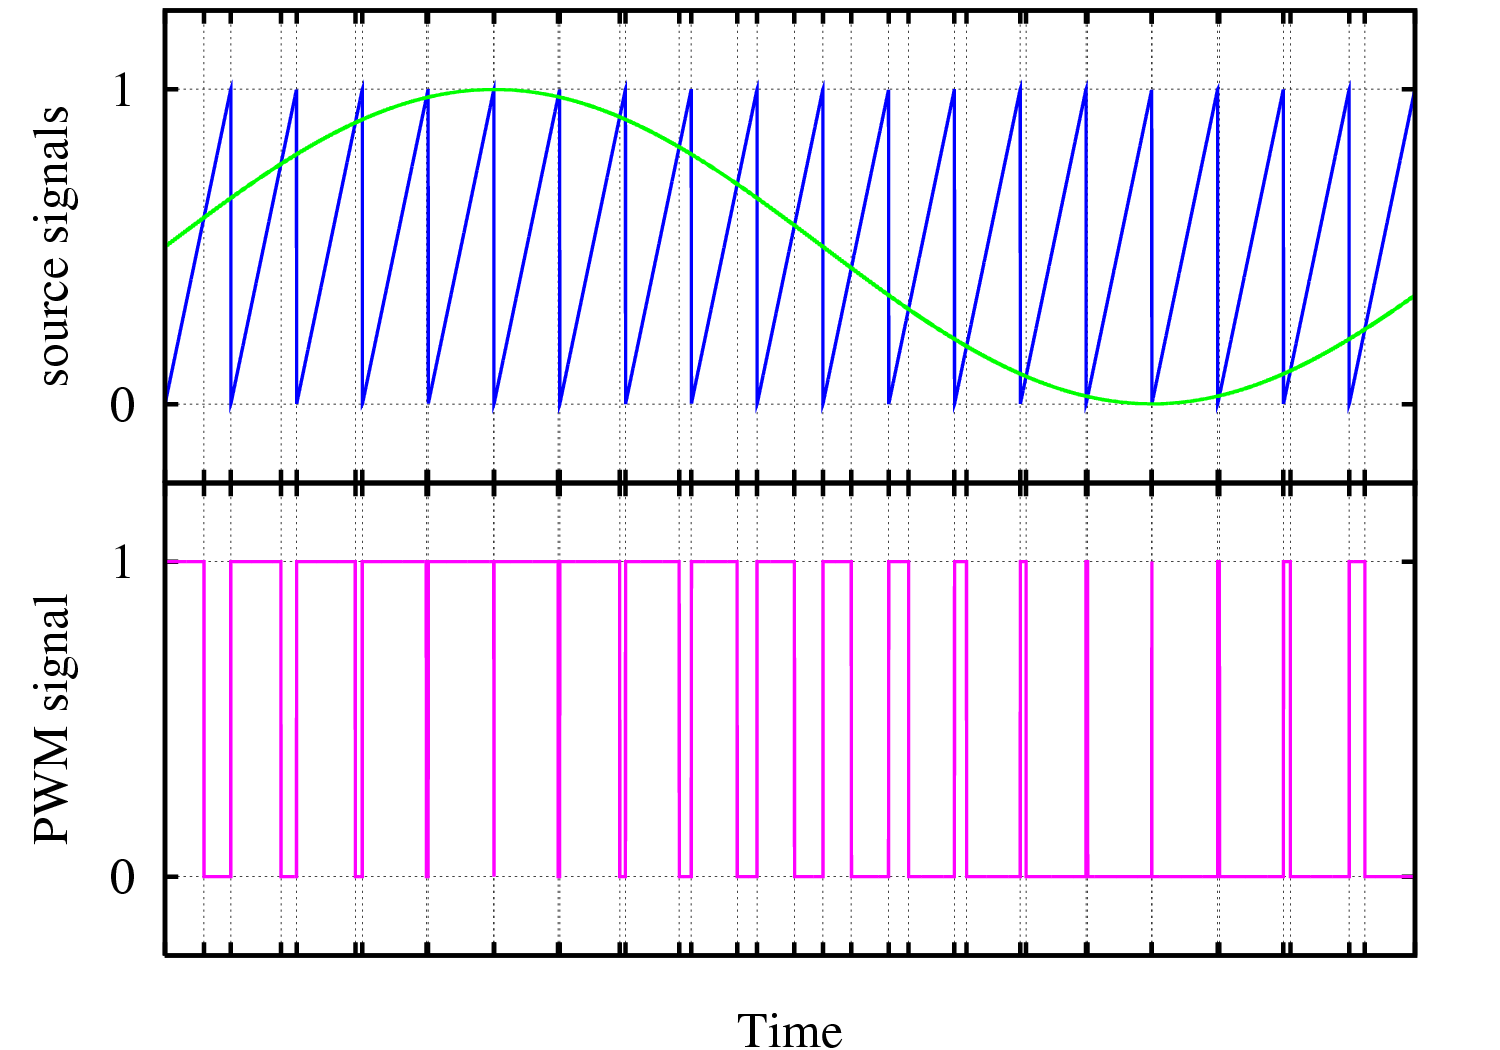
\includegraphics[width=\linewidth]{pwm}
		\end{column}
	\end{columns}
	\ccbysa{http://commons.wikimedia.org/wiki/File:Pwm.png}{CyrilB}
\end{frame}

\begin{frame}[fragile]
	\frametitle{PWM Output}
	You can use PwmOut on any purple pin marked PWM:
	\begin{lstlisting}[numbers=none]
		PwmOut out(PinName pin);
	\end{lstlisting}
	\vfill
	\begin{columns}[T]
		\begin{column}{0.5\textwidth}
			The period is controlled with:
			\begin{lstlisting}[numbers=none]
				out.period(float seconds);
				out.period_ms(int ms);
				out.period_us(int us);
			\end{lstlisting}
			and defaults to 0.02 seconds.
		\end{column}
		\begin{column}{0.5\textwidth}
			The pulse width is controlled with:
			\begin{lstlisting}[numbers=none]
				out = 0.5;
				out.write(float value);
				out.pulsewidth(float seconds);
				out.pulsewidth_ms(int ms);
				out.pulsewidth_us(int us);
			\end{lstlisting}
			The first two methods take a float in the range [0.0 -- 1.0].
		\end{column}
	\end{columns}
	\vfill
	Use whichever methods suit your application best.
\end{frame}

\begin{frame}[fragile]
	\frametitle{PWM Demo}
	\begin{columns}[T]
		\begin{column}{0.5\textwidth}
			Create a new program:
			\begin{itemize}
				\item PwmOut connected to the LED
				\item A loop changing the brightness of the LED
				\pause
				\item Brightness is proportional to duty cycle
				\item Don't forget to slow your program down!
				\pause
				\item Try playing with the period
			\end{itemize}
		\end{column}
		\begin{column}{0.5\textwidth}
			\lstinputlisting[title=Pwm.cpp]{code/modular_code/pwm.cpp}
		\end{column}
	\end{columns}
\end{frame}

\begin{frame}
	\frametitle{PWM Notes}
	Be aware that the same PWM signal may be exposed on several pins, you can only use one at a time.
	\vfill
	PWMx/y is the y-th channel of the x-th timer. All PWM's on a single timer must have the same frequency/period but can have different duty cycles.
	\vfill
	PWMx/yN has the same period and duty cycle as PWMx/y but is inverted.
\end{frame}

\subsection{Classes}
\label{sub:classes}
\begin{frame}
	\frametitle{Classes}
	A class is an object that can contain both variables and functions.
	DigitalIn, DigitalOut and all the other objects used so far are examples of classes.\\
	\vfill
	Using classes helps you:
	\begin{itemize}
		\item Stay organized - functions are attached to the data they use
		\item Reuse code - you can make as many copies as needed without extra code
		\item Control scope - you don't have to worry about name clashes
	\end{itemize}
\end{frame}

\begin{frame}[fragile]
	\frametitle{Class Structure}
	\lstinputlisting[]{code/modular_code/class0.cpp}
\end{frame}

\begin{frame}[fragile]
	\frametitle{Class Structure}
	The {\ttfamily class} keyword defines this block as a class.
	\vfill
	The {\ttfamily public} and {\ttfamily private} keywords are access specifiers.
	Private members are only available from other members of the same class.
	Public members are available anywhere the object is.
	\vfill
	Your class becomes a new data type in your program.
	You can create instances of it and use them like any other object.
	\vfill
	Class members are accessed with dot notation: {\ttfamily name.member}
	\vfill
	Class scope can be accessed with the :: scope operator
\end{frame}

\begin{frame}[fragile]
	\frametitle{Class Scope}
	\lstinputlisting[]{code/modular_code/class1.cpp}
\end{frame}

\begin{frame}[fragile]
	\frametitle{Header Files}
	Header files allow you to separate interface from implementation:
	\begin{itemize}
		\item Interface - Class and member definition in header file (.h)
		\item Implementation - Function bodies go in source file (.cpp)
	\end{itemize}
	\vfill
	Always use include guards in your header files:
	\begin{lstlisting}[title=sample.h]
		#ifndef SAMPLE_H_
		#define SAMPLE_H_
		...
		#endif
	\end{lstlisting}
	\vfill
	Include your headers with the \texttt{\#include} directive:
	\begin{lstlisting}
		#include "sample.h"
	\end{lstlisting}
\end{frame}

\begin{frame}[fragile,squeeze]
	\frametitle{Header Files}
	\lstinputlisting[title=Rectangle.h]{code/modular_code/rectangle.h}
	\lstinputlisting[title=Rectangle.cpp]{code/modular_code/rectangle.cpp}
\end{frame}

\begin{frame}[fragile]
	\frametitle{Writing a Class}
	Lets convert this simple code into a class by following these steps:
	\begin{columns}[T]
		\begin{column}{0.5\textwidth}
			\begin{enumerate}
				\item Refactor into functions
				\bigskip
				\item Encapsulate into a class
				\bigskip
				\item Expose class with a header
			\end{enumerate}
		\end{column}
		\begin{column}{0.5\textwidth}
			\lstinputlisting[]{code/fader/fader1.cpp}
		\end{column}
	\end{columns}
\end{frame}

\begin{frame}[fragile]
	\frametitle{Refactoring}
	Pull out as much common code as you can into functions:
	\lstinputlisting[]{code/fader/fader2.cpp}
\end{frame}

\begin{frame}[fragile]
	\frametitle{Encapsulating}
	Encapsulate your code in a class by moving any relevant variables and functions into the class body:
	\begin{itemize}
		\item Variables should be private unless you have a good reason to make them public!
		\item Provide get/set functions to access needed private variables
		\item Most functions should be public
		\item Use private functions to avoid repeating yourself
	\end{itemize}
\end{frame}

\begin{frame}[fragile]
	\frametitle{Encapsulating}
	\lstinputlisting[multicols=2]{code/fader/fader3.cpp}
\end{frame}

\begin{frame}
	\frametitle{Exposure}
	%TODO
\end{frame}

\begin{frame}[fragile]
	\frametitle{Exposure}
	\begin{columns}[T]
		\begin{column}{0.5\textwidth}
			\lstinputlisting[title=Fader.h]{code/fader/Fader.h}
		\end{column}
		\begin{column}{0.5\textwidth}
			\lstinputlisting[title=Fader.cpp]{code/fader/Fader.cpp}
		\end{column}
	\end{columns}
\end{frame}

\begin{frame}
	\frametitle{Using Your Class}
	\begin{columns}[T]
		\begin{column}{0.5\textwidth}
			\begin{itemize}
				\item Create an instance of your class
				\item Invoke your class methods in your main function
				\item You can easily add more by creating more instances
			\end{itemize}
		\end{column}
		\begin{column}{0.5\textwidth}
			\lstinputlisting[title=FaderDemo.cpp]{code/fader/FaderDemo.cpp}		
		\end{column}
	\end{columns}
\end{frame}